%!TEX root = ../thesis.tex
\section{Evaluation}
\label{mixt_evaluation}

To evaluate MixT, we measure the performance of our automatic tutorial generation pipeline and gather user feedback on the effectiveness of the resulting MixT tutorials.

\subsection{Expert Inspection of Generated Results}
We examined the segmented and cropped videos for each step of our nine converted tutorials and recorded the following errors. If a clip does not include all actions of the current step, we record a \emph{segmentation error}. If the screenshots or zoom/crop videos do not show the appropriate application regions, we record a \emph{region finding error}; if the system fails to identify the active region and shows the overall UI instead, we record a \emph{region finding miss}; if they show some relevant regions but omit others, we record an \emph{incomplete region}.

Table~\ref{tab:mixt_errors} shows the results of our inspection. On average, MixT correctly segmented steps around 92\% and found relevant regions of complete views 92\% of the time. These error rates suggest that our automatic generation pipeline performs reasonably well for a variety of real-world tutorials, but there is room to improve our segmentation and region-finding accuracy.

\begin{table}
  \centering
  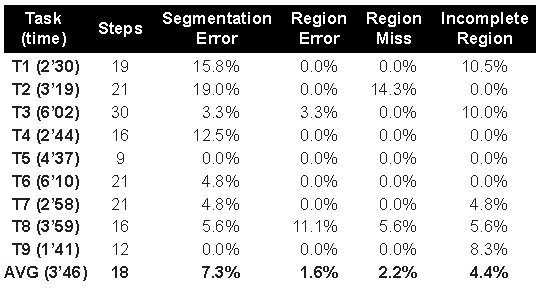
\includegraphics[width=0.5\columnwidth]{\mixt/fig/error_rates}
  \caption{Error rates for automatically generated tutorials.}
  \label{tab:mixt_errors}
\end{table}

% ---------------------------------------------------------------

\subsection{User Experiences: Working with MixT Tutorials}
We conducted a small user evaluation with four participants (2 males and 2 females, aged 25-29, with 5-12 years of Photoshop experience) to gather feedback on the usability of our MixT tutorials. We selected four of our nine evaluation tutorials with features such as the \emph{brush} tool, \emph{pen} tool, \emph{puppet warp} tool, and \emph{gradient warp} tool –- commands that led to many video views in our formative study (Table~\ref{tab:formative_video_views}). These test tutorials were generated with an earlier version of MixT that did not use the mouse event log to refine the step segmentation and active UI region finding as described earlier. This previous implementation relied solely on the command log and computer vision, which resulted in lower segmentation accuracy (84\%) and region-finding accuracy (90\%).

Participants were introduced to the MixT system and then asked to work through the set of tutorials, analogously to our formative study. We asked participants to comment on their process using the think-aloud method, and afterwards asked open-ended questions to elicit additional detail.

\subsubsection{Successes}
The participants found the same benefits in automatically-generated MixT tutorials as earlier participants found in manually-created tutorials. Participants commented that videos helped them understand steps that were complicated or text that was ambiguous or did not contain explanations why certain steps were taken: \iquote{Videos were convenient when trying to get a sense of a complex operation.} / \iquote{I tended to watch the videos when the text wasn't clear.} Examples included making a selection from a path (1.75 views per user) and the \emph{puppet warp} tool (2.75 views). Note that a clip might be viewed more than once by a single user. Participants also watched videos to confirm their results because \iquote{The photo/screenshot (...) wasn't as actively helpful in guiding what I needed to do or confirming that I was doing the right thing.}
%
Multiple participants commented positively on the utility of automatically segmented videos that focus on short step clips about the task at hand: \iquote{I didn't have to sit through 5 mins of intro to get a video description of the task I was interested in} / \iquote{What I liked the most about the mixed tutorial was the ability to only watch short segments of video that was relevant. Often with video tutorials I find myself sitting and waiting for the content that I need. Because of this, I tend to avoid video tutorials in favor of text. The mixed tutorial was a nice way to achieving the best of both worlds.}

\subsubsection{Shortcomings}
Our participants identified useful suggestions for improving our tutorial design. Currently, static images do not provide sufficient \emph{information scent} about the contents of the video – it was hard to judge how long each video was and whether there were remaining important actions in a clip. Therefore, participants sometimes skipped important information that resulted in editing errors (e.g., not adjusting the pose after placing pins using the \emph{puppet warp} tool). In addition, the minimal play/pause interface was deemed insufficient: \iquote{Navigating the videos was difficult [...] It was also hard to go back in the video to observe missed steps. Adding standard playback controls might help.} One approach to remedy this would be to analyze the video and provide thumbnail frames of the video clip that highlight the clip's content and length.

As mentioned earlier, our automatic tutorial generation pipeline computes the correct video segments and finds the right spatial regions to highlight for most steps. However, the few segmentation and region finding errors that users encountered sometimes caused important information to be hidden in crop or zoom mode. As a result, participants referred back to the normal video mode more often than we expected, even though the crop and zoom videos were typically more legible. For the 41 video segments that were watched, the average view counts per step were 0.66 for crop mode, 0.24 for zoom mode, and 1.8 for normal mode. Participants commented on the impact of segmentation errors: \iquote{Sometimes the video doesn't line up –- and you have to go to the step before to see what's going on.} We consider this as an opportunity to include the tutorial authors in the loop to modify computer-generated tutorials.
